\subsection{Grokking Phenomenon of Other Models}
\label{sec:subtask2}

We study the grokking phenomenon for two other network architectures, long short-term memory (LSTM) and multilayer perceptron (MLP), suggesting that grokking is not unique for transformer.
Specifically, our LSTM has $2$ layers, a hidden state of size $d_{\mathrm{hidden}} = 128$, and dropout $0.1$.
Our MLP has $2$ hidden layers of size $d_{\mathrm{hidden}}^{(1)} = d_{\mathrm{hidden}}^{(2)} = 256$, both of which have dropout $0.1$.
Other hyperparameters remain the same as \cref{sec:subtask1}.

The grokking curves for LSTM and MLP are shown in \cref{fig:acc_and_loss_LSTM} and \cref{fig:acc_and_loss_MLP}, respectively.

\begin{figure}[!ht]
    \centering
    \begin{subfigure}{0.45\textwidth}
        \centering
        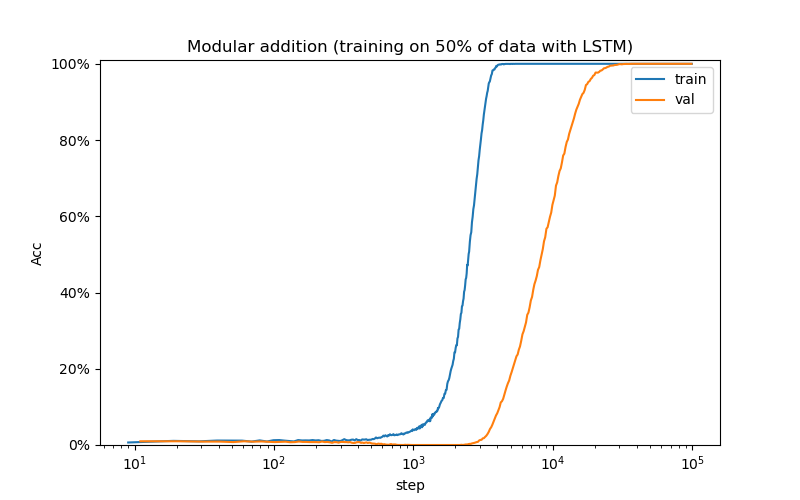
\includegraphics[width=\linewidth]{fig/grokking_curves/addition_50_LSTM_step.png}
        \caption{Training and validation accuracy}
        \label{fig:grokking_curve_LSTM}
    \end{subfigure}
    %\hfill
    \begin{subfigure}{0.45\textwidth}
        \centering
        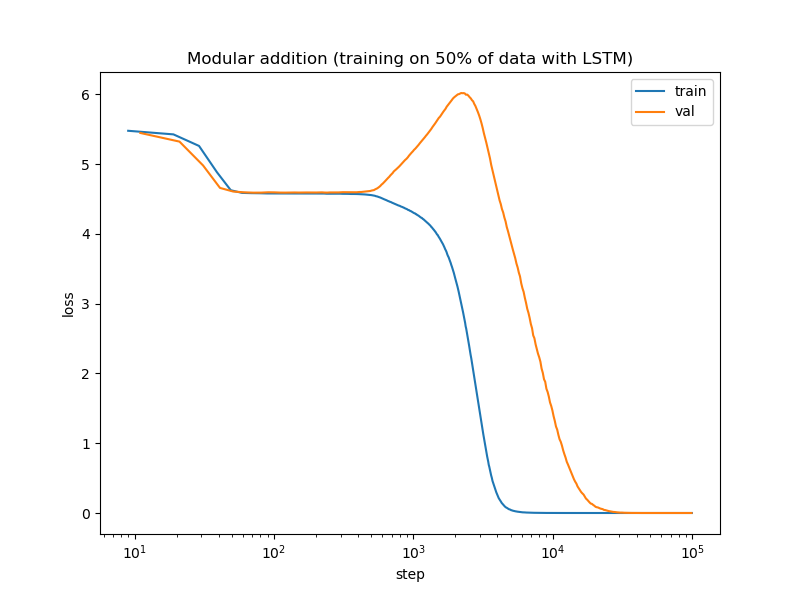
\includegraphics[width=\linewidth]{fig/loss_curves/addition_50_LSTM_step.png}
        \caption{Training and validation loss}
        \label{fig:loss_curve_LSTM}
    \end{subfigure}

    \caption{The grokking curves of LSTM model}
    \label{fig:acc_and_loss_LSTM}
\end{figure}

\begin{figure}[!ht]
    \centering
    \begin{subfigure}{0.45\textwidth}
        \centering
        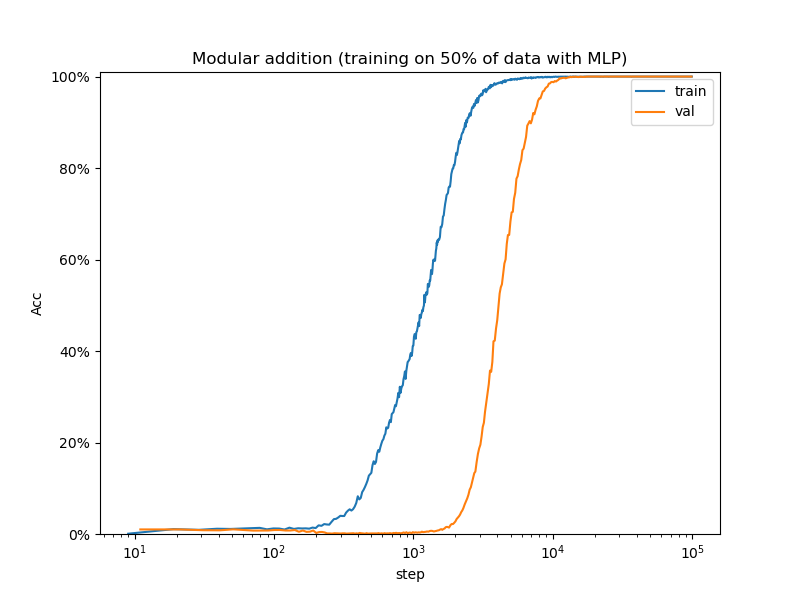
\includegraphics[width=\linewidth]{fig/grokking_curves/addition_50_MLP_step.png}
        \caption{Training and validation accuracy}
        \label{fig:grokking_curve_MLP}
    \end{subfigure}
    %\hfill
    \begin{subfigure}{0.45\textwidth}
        \centering
        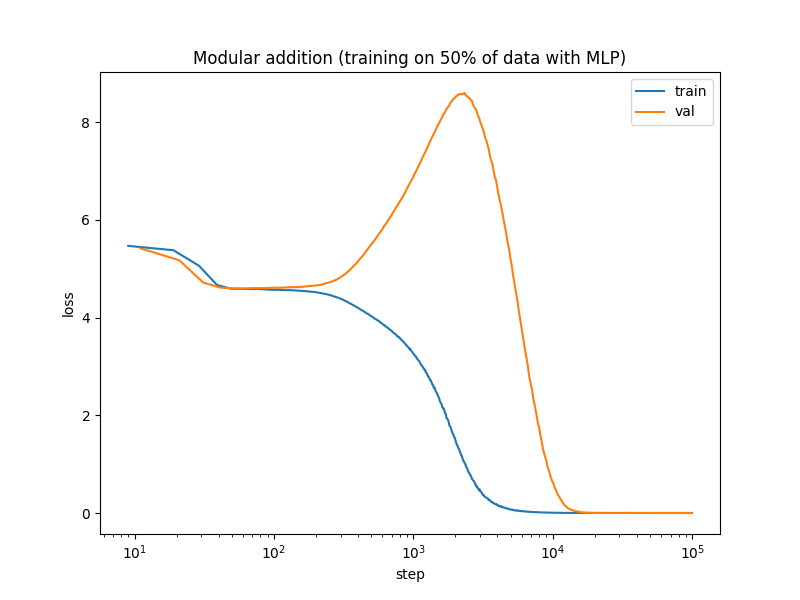
\includegraphics[width=\linewidth]{fig/loss_curves/addition_50_MLP_step.png}
        \caption{Training and validation loss}
        \label{fig:loss_curve_MLP}
    \end{subfigure}

    \caption{The grokking curves of MLP model}
    \label{fig:acc_and_loss_MLP}
\end{figure}

In \cref{fig:grokking_curve_LSTM,fig:grokking_curve_MLP}, we again observe a delay of generalization which, however, is not as significant as that in \cref{fig:grokking_curve_transformer}.
Besides, a similar increase of validation loss could be observed in both \cref{fig:loss_curve_LSTM} and \cref{fig:loss_curve_MLP}.